%
% TEXTOS SOBRE O PENSAMENTO MUSICAL
% ---------------------------------
% Agustín de Hipona (San Agustín)
%
\begin{multicols}{2}
%
%\subsection*{Pensadores e textos}\label{pensadores-textos}
%
\paragraph{Boecio (470-524): \emph{Tratado de música}}\label{Boecio-tratado}
%
Severino Boecio, o máis relevante teórico musical no tránsito á Idade Media, foi un alto funcionario da corte ostrogoda, que terminou condenado á morte polo rei Teodorico. No cárcere escribiu a súa obra máis famosa, \emph{El consuelo de la filosofía}.\\
Boecio proxectou realizar un gran compendio das ciencias da súa época, chamadas entón artes liberais; a pesar de que non se concluíu, si redactou algúns tratados, entre eles o referido á música. Este tratado converteuse en libro de referencia de todos os teóricos musicais durante a Idade media e tamén no Renacemento, e os seus contidos foron repetidos case literalmente durante séculos.

No comezo do tratado, Boecio realiza unha clasificación das partes da música que se faría tópica posteriormente. Este é o texto que segue.
%
%\begin{figure}[h]
%\centering
%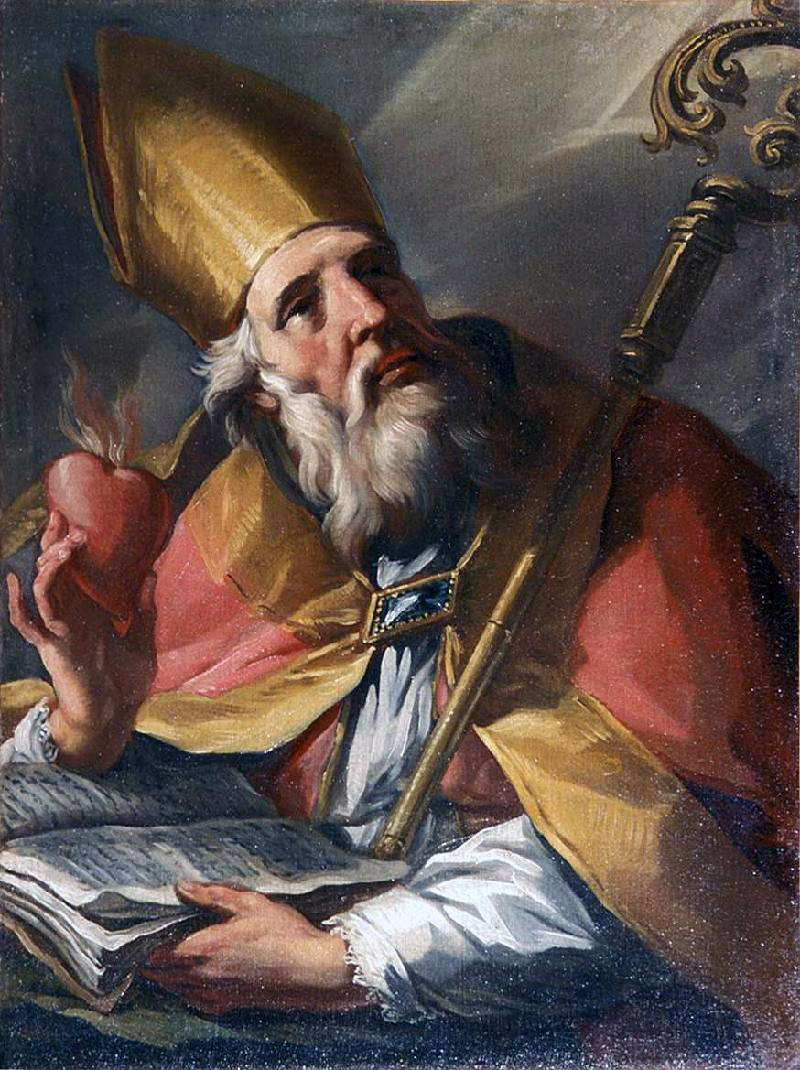
\includegraphics[width=0.5\textwidth]{ud-03/SanAgustin.jpg}
%\caption{San Agustín canonizado.\\
%(Fonte: wikimedia commons)}
%\label{fig:San-Agustin}
%\end{figure}
%
\begin{Figura}
  \centering
  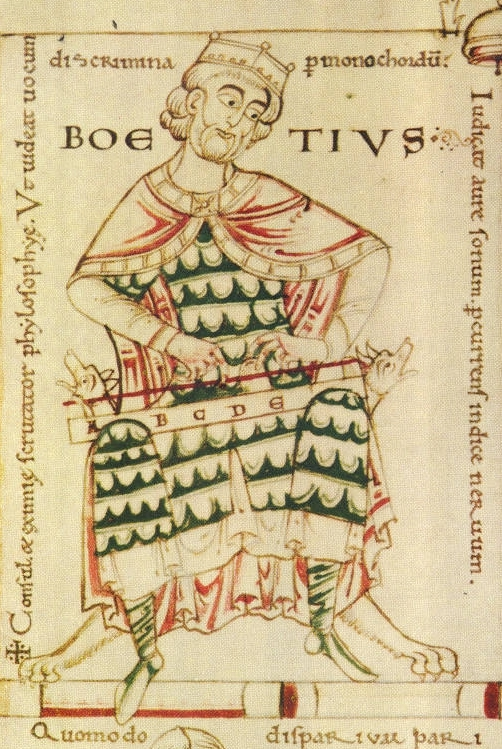
\includegraphics[width=0.75\textwidth]{ud-03/boecio.jpg}
  \captionof{figure}{Severino Boecio (470-524).\\
  (Fonte: wikimedia commons)}
  \label{fig:Severino-Boecio}
\end{Figura}
%
\end{multicols}
%
\vspace*{0.05cm}
\begin{quote}
\small{
``Aquel que escribe de música debe saber exponer en primer lugar las partes en que los estudiosos han subdividido la materia. Estas son tres: la primera está formada por la música del universo (mundana); la segunda por la música humana, y la tercera por la música instrumental, como la de la cítara, de las flautas y de los demás instrumentos con los que se puede obtener una melodía.

La música del universo, que hay que estudiar sobre todo en los cielos, es resultado de la unión de los elementos o de la variación de las estaciones. ¿Cómo podría moverse en carrera muda y silenciosa el mecanismo del cielo tan veloz? A pesar de que tal sonido no llegue a nuestro oído —y ello sucede necesariamente por múltiples razones— el movimiento rapidísimo de cuerpos tan enormes no puede darse sin sonido alguno, especialmente porque los movimientos orbitales de los astros están vinculados en una relación tan perfecta que no se puede imaginar nada más compacto y proporcionado. En efecto, algunos se mueven más arriba y otros más abajo, girando todos ellos con un impulso tan bien combinado que sus diferentes velocidades dan lugar a un orden racional en los movimientos. Por ello no puede ser ajeno a este movimiento rotatorio de los cielos el orden racional en la modulación de los sonidos. [...]

Todos pueden comprender lo que significa la música humana examinándose a sí mismos. En efecto, ¿qué une al cuerpo la incorpórea vitalidad de la mente sino una relación ordenada, como si se tratase de una justa combinación de sonidos graves y agudos para producir una única consonancia? Además, ¿qué podría asociar entre sí las partes del alma, la cual —según la doctrina de Aristóteles— es resultado de la fusión de lo irracional con lo racional? Y también: ¿qué podría mezclar los elementos del cuerpo y combinar sus partes con una relación ordenada? Pero de esto también trataremos más adelante.

La tercera parte de la música es la que se considera propia de algunos instrumentos. Es producida por la tensión, como en la cuerda; por el aire, como en las flautas, o en otros instrumentos activados por el agua; por la percusión, como en los instrumentos cuya concavidad es golpeada con una maza de bronce, dando lugar a sonidos diversos.''
}
\end{quote}
%
\begin{ejercicio}[Pensamento musical Idade Media]
  \begin{enumerate}[1.-]
  \item
    En que época das que coñeces da Idade Media desenvolve no seu tratado as ideas sobre a música Boecio? \ldots
%    \vspace*{0.5cm}
  \item
    Sinala no texto aquelas palabras que destacarías sobre a concepción da música de Boecio. \\
    A que se refire Boecio cando fala no texto de <<música humana>>, <<música mundana>> e <<música do universo>>? Xustifica a túa resposta.
    \vspace*{6.10cm}
  \end{enumerate}
\end{ejercicio}
